\documentclass[sigplan,10pt]{acmart}

\usepackage{tikz}
\usetikzlibrary{arrows.meta}

\setcopyright{rightsretained}
\copyrightyear{2020}
\acmYear{2020}
\acmDOI{}
\acmConference[]{}{}{}
\acmBooktitle{}
\acmPrice{}
\acmISBN{}

\hyphenation{da-ta-cen-ter da-ta-cen-ters time-stamp time-stamps time-stamped hard-links}

\begin{document}
\title{Reordering Elements in List CRDTs}

\author{Martin Kleppmann}
\email{mk428@cl.cam.ac.uk}
\orcid{0000-0001-7252-6958}
\affiliation{%
  \institution{Department of Computer Science and Technology}
  \streetaddress{15 JJ Thomson Avenue}
  \city{Cambridge}
  \state{}
  \postcode{CB3 0FD}
  \country{United Kingdom}
}

\begin{abstract}
    List CRDTs (Conflict-free Replicated Data Types) allow multiple users to concurrently insert and delete items in a shared list.
    However, existing algorithms behave poorly when users concurrently reorder items in the list, or move items to a new position.
    We describe an extension to list CRDTs that improves their support for reordering.
\end{abstract}

\settopmatter{printfolios=true} % Recommended EuroSys formatting
\maketitle

\section{Introduction}

Conflict-free Replicated Data Types (CRDTs) allow multiple replicas to concurrently modify some shared data object, while ensuring that all replicas eventually converge towards the same, consistent state~\cite{Shapiro:2011un}.
CRDT algorithms have been developed for various different datatypes, and one of the most important datatypes is the \emph{list} (also called \emph{sequence} or \emph{array} datatype).
A list is a collection of elements in a total order, which is chosen by the user.

Replicated lists can be used to implement a variety of important applications, such as:
\begin{itemize}
    \item text editors (text is a list of characters);
    \item graphics applications (a list of graphical objects, where the order determines visibility: objects ``further down'' may be occluded or filtered by the objects ``higher up'', as illustrated in Fig.~\ref{fig:smiley});
    \item to-do lists and task trackers (a list of tasks, where the order may reflect the relative priority of tasks as chosen by the user).
\end{itemize}

\begin{figure*}
  \centering
  \includegraphics{smiley.pdf}
  \caption{Graphics software often places objects in a list that determines the z-index; objects higher in the list occlude lower ones. %
    Here, the eyeballs and mouth are placed above the yellow face, and the pupils in turn are placed above the eyeballs.}
  \label{fig:smiley}
\end{figure*}

Many list CRDTs have been developed, such as WOOT~\cite{Oster:2006wj}, Treedoc~\cite{Preguica:2009fz}, RGA~\cite{Roh:2011dw}, Causal Trees/Timestamped Insertion Trees~\cite{Grishchenko:2014eh,Attiya:2016kh}, Logoot \cite{Weiss:2009ht,Weiss:2010hx}, and LSEQ \cite{Nedelec:2013ky,Nedelec:2016eo}.
Moreover, most of the field of Operational Transformation algorithms is dedicated to algorithms for collaboratively editable text, i.e.\ lists~\cite{Ellis:1989ue,Nichols:1995fd,Ressel:1996wx,Sun:1998vf,Oster:2006tr}.

All of the aforementioned algorithms allow replicas to \emph{insert} or \emph{delete} elements anywhere in the list.
However, none of them have explicit support for \emph{reordering} or \emph{moving} elements from one position to another position in the list.
This is a surprising omission because reordering is a commonly required operation: in many to-do list applications, a user can drag and drop list elements to reorder them, and graphics software allows users to reorder the object list with commands such as ``bring to front'' (which moves an object to the top of the list) and ``send to back'' (which moves an object to the bottom).

In this paper we introduce an algorithm that allows an existing list CRDT to be extended with a reorder operation.
The algorithm is generic in the sense that it can be implemented on top of any of the aforementioned list CRDTs.

\section{Semantics of Concurrent Moves}\label{sec:semantics}

The simplest way of moving a list element is to delete it from its existing position, and to re-insert it at the new position.
However, if two replicas concurrently move the same element, the result is that the element is duplicated: the two deletions of the same element behave the same as one deletion, and the two insertions independently re-insert the element twice.

\begin{figure*}
    \centering
    \vspace{3em}
    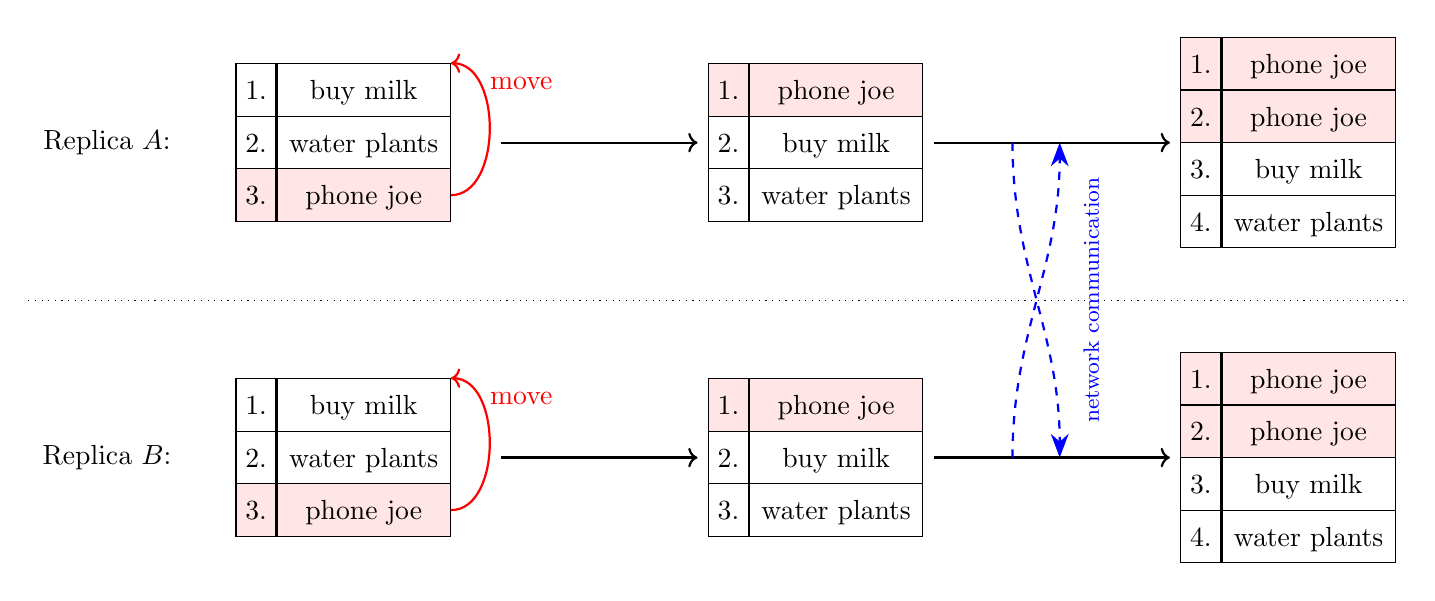
\begin{tikzpicture}[auto,scale=1.0]
        \tikzstyle{item}=[rectangle,draw,inner ysep=4pt,text height=9pt,text depth=2pt,minimum width=2.2cm]
        \tikzstyle{network}=[thick,dashed,blue,-{Stealth[length=3mm]}]
        \path [draw,dotted] (0,2) -- (17.5,2);
        \node at (1, 4) {Replica $A$:};
        \node at (1, 0) {Replica $B$:};
        \matrix [row sep={19pt,between origins},nodes=item] at (4, 4) {
            \node [minimum width=0.5cm] {1.}; & \node (top1) {buy milk}; \\
            \node [minimum width=0.5cm] {2.}; & \node {water plants}; \\
            \node [minimum width=0.5cm,fill=red!10] {3.}; & \node [fill=red!10] (joe1) {phone joe}; \\
        };
        \matrix [row sep={19pt,between origins},nodes=item] at (4, 0) {
            \node [minimum width=0.5cm] {1.}; & \node (top2) {buy milk}; \\
            \node [minimum width=0.5cm] {2.}; & \node {water plants}; \\
            \node [minimum width=0.5cm,fill=red!10] {3.}; & \node [fill=red!10] (joe2) {phone joe}; \\
        };
        \draw [->,red,thick] (joe1.east) to [in=0, out=0] node [right,near end] {move} (top1.north east);
        \draw [->,red,thick] (joe2.east) to [in=0, out=0] node [right,near end] {move} (top2.north east);
        \draw [->,thick] (6, 0) -- (8.5, 0);
        \draw [->,thick] (6, 4) -- (8.5, 4);
        \matrix [row sep={19pt,between origins},nodes=item] at (10, 4) {
            \node [minimum width=0.5cm,fill=red!10] {1.}; & \node [fill=red!10] {phone joe}; \\
            \node [minimum width=0.5cm] {2.}; & \node {buy milk}; \\
            \node [minimum width=0.5cm] {3.}; & \node {water plants}; \\
        };
        \matrix [row sep={19pt,between origins},nodes=item] at (10, 0) {
            \node [minimum width=0.5cm,fill=red!10] {1.}; & \node [fill=red!10] {phone joe}; \\
            \node [minimum width=0.5cm] {2.}; & \node {buy milk}; \\
            \node [minimum width=0.5cm] {3.}; & \node {water plants}; \\
        };
        \draw [->,thick] (11.5, 0) -- (14.5, 0);
        \draw [->,thick] (11.5, 4) -- (14.5, 4);
        \draw [network] (12.5, 0) to [out=90,in=270] (13.1, 4);
        \draw [network] (12.5, 4) to [out=270,in=90] (13.1, 0);
        \node [rotate=90,blue,font=\footnotesize] at (13.5, 2) {network communication};
        \matrix [row sep={19pt,between origins},nodes=item] at (16, 4) {
            \node [minimum width=0.5cm,fill=red!10] {1.}; & \node [fill=red!10] {phone joe}; \\
            \node [minimum width=0.5cm,fill=red!10] {2.}; & \node [fill=red!10] {phone joe}; \\
            \node [minimum width=0.5cm] {3.}; & \node {buy milk}; \\
            \node [minimum width=0.5cm] {4.}; & \node {water plants}; \\
        };
        \matrix [row sep={19pt,between origins},nodes=item] at (16, 0) {
            \node [minimum width=0.5cm,fill=red!10] {1.}; & \node [fill=red!10] {phone joe}; \\
            \node [minimum width=0.5cm,fill=red!10] {2.}; & \node [fill=red!10] {phone joe}; \\
            \node [minimum width=0.5cm] {3.}; & \node {buy milk}; \\
            \node [minimum width=0.5cm] {4.}; & \node {water plants}; \\
        };
    \end{tikzpicture}
    \caption{If reordering is implemented by deleting and re-inserting, concurrent moves of the same item result in the anomaly shown here: the moved item is duplicated.}
    \label{fig:duplication}
\end{figure*}

\begin{figure*}
    \centering
    \vspace{3em}
    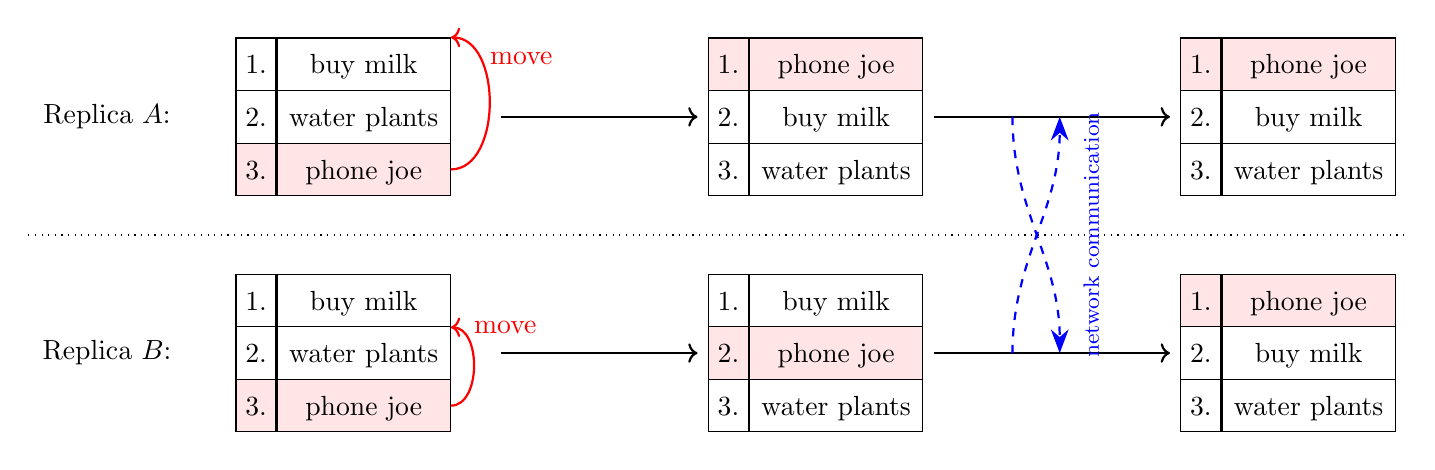
\begin{tikzpicture}[auto,scale=1.0]
        \tikzstyle{item}=[rectangle,draw,inner ysep=4pt,text height=9pt,text depth=2pt,minimum width=2.2cm]
        \tikzstyle{network}=[thick,dashed,blue,-{Stealth[length=3mm]}]
        \path [draw,dotted] (0,1.5) -- (17.5,1.5);
        \node at (1, 3) {Replica $A$:};
        \node at (1, 0) {Replica $B$:};
        \matrix [row sep={19pt,between origins},nodes=item] at (4, 3) {
            \node [minimum width=0.5cm] {1.}; & \node (top1) {buy milk}; \\
            \node [minimum width=0.5cm] {2.}; & \node {water plants}; \\
            \node [minimum width=0.5cm,fill=red!10] {3.}; & \node [fill=red!10] (joe1) {phone joe}; \\
        };
        \matrix [row sep={19pt,between origins},nodes=item] at (4, 0) {
            \node [minimum width=0.5cm] {1.}; & \node (top2) {buy milk}; \\
            \node [minimum width=0.5cm] {2.}; & \node {water plants}; \\
            \node [minimum width=0.5cm,fill=red!10] {3.}; & \node [fill=red!10] (joe2) {phone joe}; \\
        };
        \draw [->,red,thick] (joe1.east) to [in=0, out=0] node [right,near end] {move} (top1.north east);
        \draw [->,red,thick] (joe2.east) to [in=0, out=0] node [right,at end,inner xsep=8pt] {move} (top2.south east);
        \draw [->,thick] (6, 0) -- (8.5, 0);
        \draw [->,thick] (6, 3) -- (8.5, 3);
        \matrix [row sep={19pt,between origins},nodes=item] at (10, 3) {
            \node [minimum width=0.5cm,fill=red!10] {1.}; & \node [fill=red!10] {phone joe}; \\
            \node [minimum width=0.5cm] {2.}; & \node {buy milk}; \\
            \node [minimum width=0.5cm] {3.}; & \node {water plants}; \\
        };
        \matrix [row sep={19pt,between origins},nodes=item] at (10, 0) {
            \node [minimum width=0.5cm] {1.}; & \node {buy milk}; \\
            \node [minimum width=0.5cm,fill=red!10] {2.}; & \node [fill=red!10] {phone joe}; \\
            \node [minimum width=0.5cm] {3.}; & \node {water plants}; \\
        };
        \draw [->,thick] (11.5, 0) -- (14.5, 0);
        \draw [->,thick] (11.5, 3) -- (14.5, 3);
        \draw [network] (12.5, 0) to [out=90,in=270] (13.1, 3);
        \draw [network] (12.5, 3) to [out=270,in=90] (13.1, 0);
        \node [rotate=90,blue,font=\footnotesize] at (13.5, 1.5) {network communication};
        \matrix [row sep={19pt,between origins},nodes=item] at (16, 3) {
            \node [minimum width=0.5cm,fill=red!10] {1.}; & \node [fill=red!10] {phone joe}; \\
            \node [minimum width=0.5cm] {2.}; & \node {buy milk}; \\
            \node [minimum width=0.5cm] {3.}; & \node {water plants}; \\
        };
        \matrix [row sep={19pt,between origins},nodes=item] at (16, 0) {
            \node [minimum width=0.5cm,fill=red!10] {1.}; & \node [fill=red!10] {phone joe}; \\
            \node [minimum width=0.5cm] {2.}; & \node {buy milk}; \\
            \node [minimum width=0.5cm] {3.}; & \node {water plants}; \\
        };
    \end{tikzpicture}
    \caption{When the same item is concurrently moved to different positions on different replicas, one of those positions should become the ``winning'' position as the replicas converge. In this example, replica $A$'s move operation wins.}
    \label{fig:concurrent}
\end{figure*}

We argue that such duplication in the face of concurrency is undesirable, as it is generally not the behaviour expected by users.
For example, say a user has replicas of their to-do list on their laptop and their smartphone.
They reorder items on their laptop to match new priorities, and also reorder some items on their phone while the phone is offline, as illustrated in Fig.~\ref{fig:duplication}.
Later, when the phone is online again and synchronises with the laptop, any items that were moved on both devices will be duplicated.

This behaviour is especially confusing if the same item was moved to the same position (e.g.\ to the top of the list) on both devices, in which case the duplicated items are likely to be adjacent in the final list, as in Fig.~\ref{fig:duplication} (depending on any other insertions that might have taken place).
However, even if the concurrent move operations had different destination positions, duplicating the moved item at both destinations is unlikely to be desirable behaviour in most applications.

Rather, we argue that the best semantics in this situation is for the system to pick one of the destination positions as the ``winner''; as the replicas communicate, they all converge towards a list in which the moved element is located only at the winning position, and nowhere else.
This approach is illustrated in Fig.~\ref{fig:concurrent}.
Any deterministic method of picking the winner is suitable (e.g.\ based on a priority given to each replica, or based on the timestamp of the operations).

\section{A Generic Reordering Algorithm}\label{sec:algorithm}

Intuitively, if we want to pick one winner from among several concurrent moves for the same element, we can use a long-established CRDT: a last-writer wins (LWW) register~\cite{Shapiro:2011wy,Johnson:1975we}.
We need one such register for each list element, containing the position of that element.
Moving an element to a new location is then merely a matter of updating the value of that element's register.

In general, we could also use a multi-value (MV) register~\cite{Shapiro:2011wy}, which would allow an element to exist at multiple positions in the list simultaneously after having experienced conflicting moves.
This is not the same as the duplication described in Section~\ref{sec:semantics}, since the multiple positions still belong to the same element, and a subsequent move would collapse them back into a single position again.
The MV register option can be used if the LWW behaviour (discarding all but one of the concurrent moves of the same element) is unacceptable.

Regardless of whether a LWW or MV register is used, this approach requires a stable way of referencing some position in the list (i.e.\ the value held by the register).
An integer index is not suitable, because an insertion or deletion at any position would require changing all of the indices following that position.
Fortunately, all known list CRDTs already incorporate schemes for stable position identifiers.
The details vary: Treedoc uses a path through a binary tree~\cite{Preguica:2009fz}, Logoot uses a list of (integer, replicaID) pairs~\cite{Weiss:2009ht}, RGA uses a so-called s4vector~\cite{Roh:2011dw}, Causal Trees/Timestamped Insertion Trees use a timestamp~\cite{Grishchenko:2014eh,Attiya:2016kh}, and so on.
But all of these approaches have in common that they can uniquely refer to a particular position in a list, in a way that is not affected by operations on other list positions.

Assume now that $p_1, p_2, \dots$ are position identifiers according to one of the aforementioned schemes.
We can now model the state of the list as a set of $(\mathit{value}, \mathit{register})$ pairs contained in an add-wins set CRDT:
\begin{align*}
\mathit{state} = \mathrm{AWSet}(\{ & (v_1, \mathrm{LWWRegister}(p_1)),\\
    & (v_2, \mathrm{LWWRegister}(p_2)), \;\dots\})
\end{align*}
In some schemes (such as Treedoc, Logoot and LSEQ), the position identifiers themselves encode their relative ordering~\cite{Interleaving}, and thus no further state is required.
In others (such as RGA and CT), the list CRDT requires an additional data structure that determines the order in which position identifiers appear in the list.

In order to iterate over the current state of the list, we need to query the above set by the position identifiers stored within the registers.
We can do this efficiently by using a database index, which allows us to find all the tuples within a set that contain a certain value (or range of values).

Note that when the position of a list element is changed, the old position identifier no longer has any value associated with it, and thus it should be regarded as nonexistent (like a tombstone in some CRDTs).
It is also possible for multiple list elements to have the same position identifier, and thus for several list elements to appear at the same position.
This situation is similar to having a multi-value register of values at each list position.
(Note this situation is different from our earlier use of a MV register, which was about one element having multiple positions, not one position having multiple elements.)

We can avoid having multiple list elements with the same position identifier by always creating a fresh position identifier as the destination of a move operation.
All of the aforementioned list CRDTs have methods of creating new position identifiers that are guaranteed to be globally unique.

\begin{acks}
Martin Kleppmann is supported by a Leverhulme Trust Early Career Fellowship and by the Isaac Newton Trust.
\end{acks}

\bibliographystyle{ACM-Reference-Format}
\bibliography{references}{}
\end{document}
